\documentclass[tikz,border=6mm]{standalone}
\usepackage[T1]{fontenc}
\usepackage[utf8]{inputenc}
\usepackage{lmodern}
\usepackage{xcolor}
\usetikzlibrary{calc,positioning,fit}

\definecolor{ElectricBlue}{HTML}{1F6FFF}
\definecolor{NvidiaGreen}{HTML}{76B900}
\definecolor{Ink}{HTML}{1F2933}
\definecolor{Grid}{HTML}{586779}
\definecolor{ThinGrid}{HTML}{8A97A5}
\definecolor{PanelBlue}{HTML}{EDF5FF}
\definecolor{PanelGreen}{HTML}{F1F8E8}

% Paleta arcoíris pastel, una por cada par de números.
\definecolor{pair0}{HTML}{F5B5B5}
\definecolor{pair1}{HTML}{F5C2B5}
\definecolor{pair2}{HTML}{F5D1B5}
\definecolor{pair3}{HTML}{F5DFB5}
\definecolor{pair4}{HTML}{F5ECB5}
\definecolor{pair5}{HTML}{EEF5B5}
\definecolor{pair6}{HTML}{DFF5B5}
\definecolor{pair7}{HTML}{D0F5B5}
\definecolor{pair8}{HTML}{C1F5B5}
\definecolor{pair9}{HTML}{B5F5BB}
\definecolor{pair10}{HTML}{B5F5CA}
\definecolor{pair11}{HTML}{B5F5D9}
\definecolor{pair12}{HTML}{B5F5E8}
\definecolor{pair13}{HTML}{B5F2F5}
\definecolor{pair14}{HTML}{B5E4F5}
\definecolor{pair15}{HTML}{B5D5F5}
\definecolor{pair16}{HTML}{B5C7F5}
\definecolor{pair17}{HTML}{B5B8F5}
\definecolor{pair18}{HTML}{C2B5F5}
\definecolor{pair19}{HTML}{D0B5F5}
\definecolor{pair20}{HTML}{DEB5F5}
\definecolor{pair21}{HTML}{ECB5F5}
\definecolor{pair22}{HTML}{F5B5F3}
\definecolor{pair23}{HTML}{F5B5E5}
\definecolor{pair24}{HTML}{F5B5D7}
\definecolor{pair25}{HTML}{F5B5C9}
\definecolor{pair26}{HTML}{F5B5BC}
\definecolor{pair27}{HTML}{F5BBB5}
\definecolor{pair28}{HTML}{F5C8B5}
\definecolor{pair29}{HTML}{F5D6B5}
\definecolor{pair30}{HTML}{F5E4B5}
\definecolor{pair31}{HTML}{F5F1B5}

\newcommand{\cellsize}{0.60}

\begin{document}
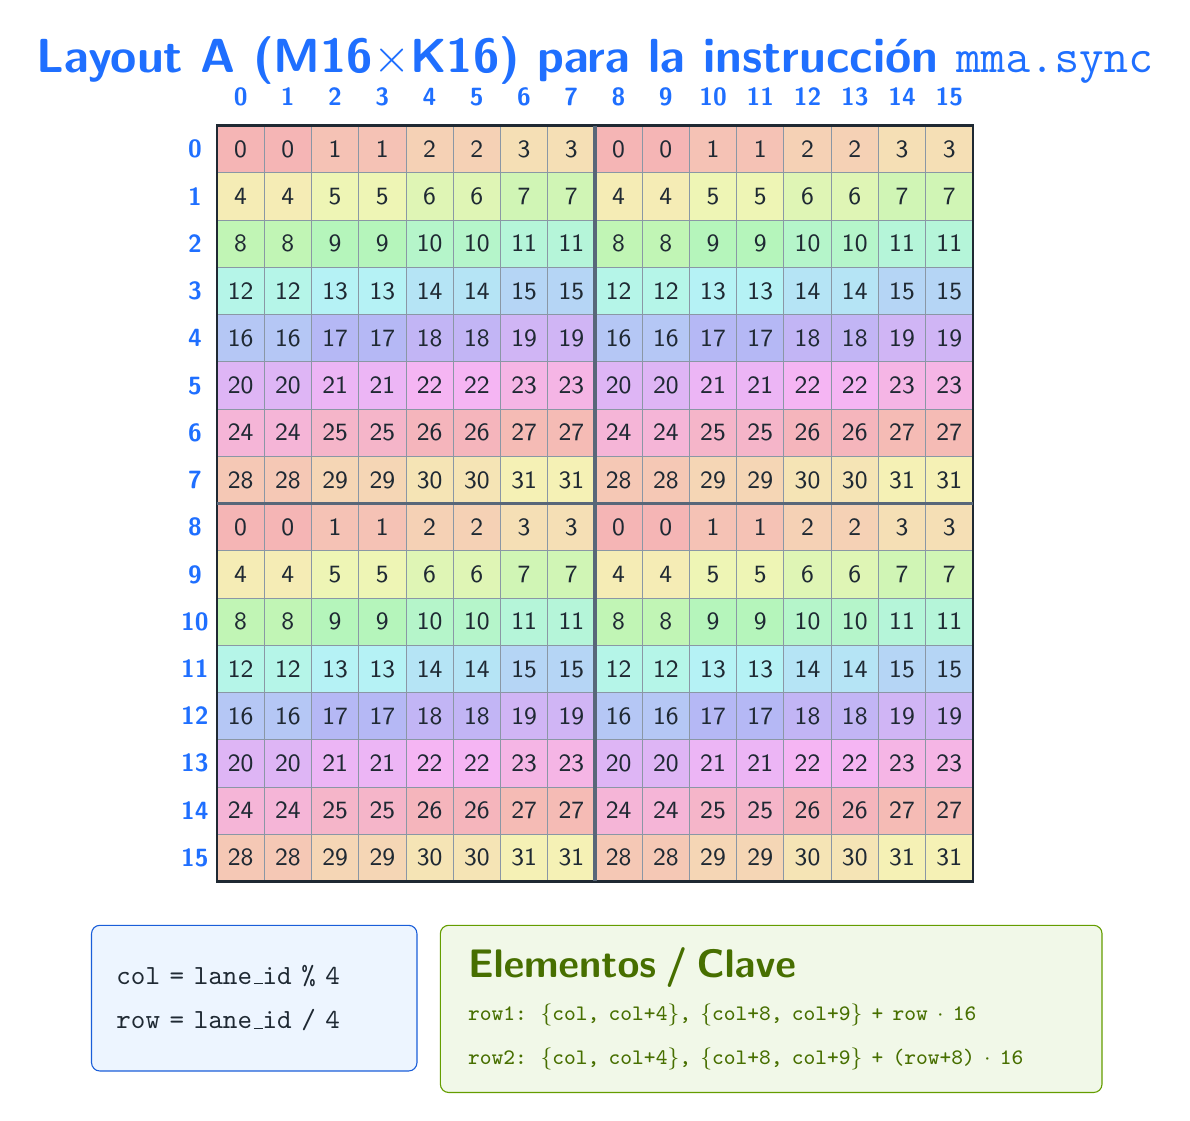
\begin{tikzpicture}[x=1cm,y=1cm]

  % Ancho total de la composición y desplazamiento para centrar la matriz.
  \def\totalwidth{12.8}
  \def\matrixwidth{9.6}
  \def\xoff{1.6}

  % Título centrado respecto a toda la figura.
  \node[anchor=north,font=\sffamily\bfseries\LARGE,text=ElectricBlue,align=center]
    at ({\totalwidth/2},0.15)
    {Layout A (M16$\times$K16) para la instrucción \texttt{mma.sync}};

  % Matriz 16x16, centrada dentro del ancho total.
  \foreach \r in {0,...,15}{
    \foreach \c in {0,...,15}{
      \pgfmathtruncatemacro{\val}{4*mod(\r,8)+floor(mod(\c,8)/2)}
      \edef\cellcolor{pair\val}
      \pgfmathsetmacro{\xA}{\xoff+\cellsize*\c}
      \pgfmathsetmacro{\xB}{\xoff+\cellsize*(\c+1)}
      \pgfmathsetmacro{\yA}{-1.10-\cellsize*\r}
      \pgfmathsetmacro{\yB}{-1.10-\cellsize*(\r+1)}
      \path[fill=\cellcolor] (\xA,\yA) rectangle (\xB,\yB);
      \draw[ThinGrid,line width=0.32pt] (\xA,\yA) rectangle (\xB,\yB);
      \node[font=\sffamily\small,text=Ink] at ({(\xA+\xB)/2},{(\yA+\yB)/2}) {\val};
    }
  }

  % Separadores gruesos 8x8 y borde exterior.
  \draw[Ink,line width=0.95pt]
    (\xoff,-1.10) rectangle ({\xoff+16*\cellsize},{-1.10-16*\cellsize});
  \draw[Grid,line width=1.35pt]
    ({\xoff+8*\cellsize},-1.10) -- ({\xoff+8*\cellsize},{-1.10-16*\cellsize});
  \draw[Grid,line width=1.35pt]
    (\xoff,{-1.10-8*\cellsize}) -- ({\xoff+16*\cellsize},{-1.10-8*\cellsize});

  % Índices de columnas y filas.
  \foreach \c in {0,...,15}{
    \pgfmathsetmacro{\xc}{\xoff+\cellsize*(\c+0.5)}
    \node[font=\sffamily\bfseries\small,text=ElectricBlue] at (\xc,-0.74) {\c};
  }
  \foreach \r in {0,...,15}{
    \pgfmathsetmacro{\yr}{-1.10-\cellsize*(\r+0.5)}
    \node[font=\sffamily\bfseries\small,text=ElectricBlue] at ({\xoff-0.28},\yr) {\r};
  }

  % Notas inferiores: nodos con ancho de texto fijo para que nada sobresalga.
  \node[
    anchor=north west,
    rounded corners=3pt,
    draw=ElectricBlue!85!black,
    fill=PanelBlue,
    text width=3.50cm,
    minimum height=1.85cm,
    inner xsep=9pt,
    inner ysep=8pt,
    font=\ttfamily\normalsize,
    text=Ink,
    align=left
  ] (boxL) at (0,-11.25)
  {col = lane\_id \% 4\\[4pt]row = lane\_id / 4};

  \node[
    anchor=north west,
    rounded corners=3pt,
    draw=NvidiaGreen!85!black,
    fill=PanelGreen,
    text width=7.70cm,
    minimum height=1.85cm,
    inner xsep=10pt,
    inner ysep=8pt,
    text=Ink,
    align=left
  ] (boxR) at (4.43,-11.25)
  {\sffamily\bfseries\Large\color{NvidiaGreen!60!black} Elementos / Clave\\[5pt]
   \ttfamily\footnotesize
   row1: \{col, col+4\}, \{col+8, col+9\} + row $\cdot$ 16\\[4pt]
   row2: \{col, col+4\}, \{col+8, col+9\} + (row+8) $\cdot$ 16};

\end{tikzpicture}
\end{document}
